%Phys24_HW1_Zih-Yu_Hsieh.tex

\documentclass{article}
\usepackage{graphicx} % Required for inserting images
\usepackage[margin = 2.54cm]{geometry}
\usepackage[most]{tcolorbox}

\newtcolorbox{myBox}[3]{
arc=5mm,
lower separated=false,
fonttitle=\bfseries,
%colbacktitle=green!10,
%coltitle=green!50!black,
enhanced,
attach boxed title to top left={xshift=0.5cm,
        yshift=-2mm},
colframe=blue!50!black,
colback=blue!10
}

\usepackage{amsmath}
\usepackage{amssymb}
\usepackage{verbatim}
\usepackage[utf8]{inputenc}
%\linespread{1.5}
\usepackage{fancyhdr}

\newtheorem{definition}{Definition}
\newtheorem{proposition}{Proposition}
\newtheorem{theorem}{Theorem}
\newtheorem{question}{Question}

\title{Phys 24 HW1}
\author{Zih-Yu Hsieh}

\fancypagestyle{plain}{%
   \fancyhead[L]\textbf{Hsieh}
   \renewcommand{\headrulewidth}{0pt}
}

\begin{document}

\maketitle

\section*{1}
\begin{myBox}[]{}
    \begin{question}
        A particle of charge $q$ and rest mass $m$ is moving with velocity $\bar{v}$
        where the magnetic field is $\bar{B}$. Here $\bar{B}$ is perpendicular to $\bar{v}$, and
        there is no electric field. Show that the path of the particle is a
        curve with radius of curvature $R$ given by $R = p/qB$, where $p$ is the
        momentum of the particle, $mv$. 
        
        (Hint: Note that the force $q\bar{v}\times\bar{B}$
        can only change the direction of the momentum, not the magni-
        tude. By what angle $\theta$ is the direction of $\bar{p}$ changed in a short time $t$?) 
        
        If $\bar{B}$ is the same everywhere, the particle will follow a
        circular path. Find the time required to complete one revolution.
    \end{question}
\end{myBox}

\textbf{Pf:}

\textbf{Radius of Curvature:}

Given particle with mass $m$, charge $q$, velocity $\bar{v}$ passing through the magnetic field $\bar{B}$ that's orthogonal to the velocity.
Which, the magenetic force exerts on the particle is $\bar{F_m} = q\bar{v}\times \bar{B}$, which the force is orthogonal to $\bar{v}$ (also the acceleration $\bar{a}=\frac{\bar{F_m}}{m}$).

Then, the unit tangent vector $\bar{T}=\bar{v}/v$, which the derivative is given by:
$$\frac{d\bar{T}}{dt} = \frac{\frac{d\bar{v}}{dt}v - \frac{dv}{dt}\bar{v}}{v^2} = \frac{v\bar{a}}{v^2} = \frac{\bar{a}}{v}$$
(Note: since $v = \sqrt{v_x^2+v_y^2+v_z^2}$, then $\frac{dv}{dt}=\frac{2(v_x\frac{dv_x}{dt}+v_y\frac{dv_y}{dt}+v_z\frac{dv_z}{dt})}{2\sqrt{v_x^2+v_y^2+v_z^2}} = \frac{\bar{v}\cdot\bar{a}}{v}$, and since $\bar{v},\bar{a}$ are orthogonal, the dot product is 0).
So, $\left\|\frac{d\bar{T}}{dt}\right\|=\frac{a}{v}$. Which, the curvature is given as follow:
$$\mathcal{K}=\frac{1}{R}=\left\|\frac{d\bar{T}}{dt}\right\|/\left\|\frac{d\bar{r}}{dt}\right\| = \frac{a/v}{\|\bar{v}\|} = \frac{a}{v^2}$$
Notice that since $\bar{F_m} = q\bar{v}\times \bar{B}$, the $F_m = \|q\bar{v}\times \bar{B}\| = qvB$ (since $\bar{v},\bar{B}$ are orthogonal), thus $a = \frac{F_m}{m} = \frac{qvB}{m}$.

So, the radius of curvature is given as:
$$R = \frac{1}{a/v^2} = \frac{v^2}{qvB/m} = \frac{mv}{qB} = \frac{p}{qB}$$
(Note: Here $p=mv$, the magnitude of momentum).


\hfill

\textbf{Time for one Revolution:}

Given that the radius of curvature $R = \frac{p}{qB} = \frac{mv}{qB}$, and the path is circular, then the circumference is given by 
$C = 2\pi R = 2\pi \frac{mv}{qB}$, which since the speed is constant $v$, then the time need to complete a revolution (going through full circumference)
is given as follow:
$$T = \frac{C}{v} = \frac{1}{v}\cdot 2\pi \frac{mv}{qB} = \frac{2\pi m}{qB}$$

\break

\section*{2}
\begin{myBox}[]{}
    \begin{question}
        Three long straight parallel wires are located as shown in
        Below Figure. One wire carries current $2I $ into the paper; each of
        the others carries current $I$ in the opposite direction. What is the
        strength of the magnetic field at the point $P_1$ and at the point $P_2$?
    \end{question}

    \begin{center}
        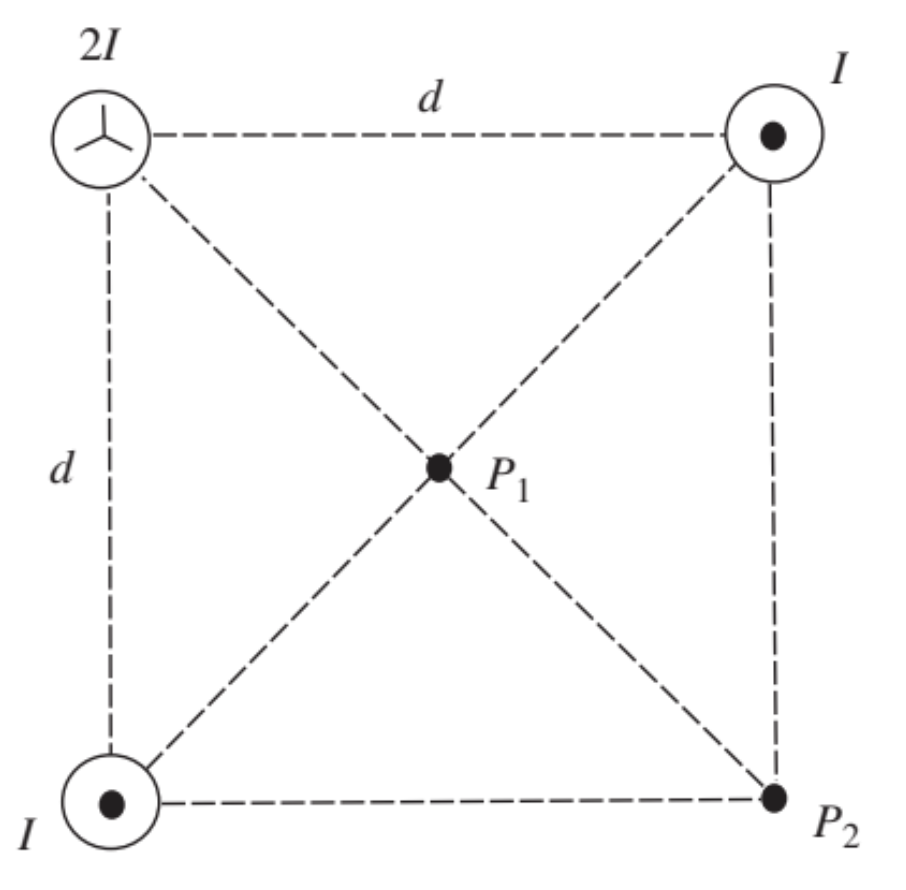
\includegraphics[width=60mm]{Figure.png}
        \label{fig:my_label}
    \end{center}
\end{myBox}

\textbf{Pf:}

For a long straight wire with current $I$ passing through, the magnetic field generated  at a point with distance $r$ radially away from the wire,
has magnitude $B=\frac{\mu_0I}{2\pi r}$, and pointing in the counterclockwise direction $\hat{\theta}$, if the current is going in the $\hat{z}$ direction in cylindrical coordinates.

Here, assume the sheet is on the xy plane (x-direction toward the right, and y-direction toward the top), while going out of the page is the z-direction.

\hfill

\textbf{Magnetic Field at $P_1$:}

First, for current $2I$ going into the plane, the direction of the field at $P_1$ is pointing toward the bottom left corner $\hat{r_1}=(-1/\sqrt{2},-1/\sqrt{2},0)$,
and the field strength is $B_1 = \frac{\mu_0\cdot 2I}{2\pi \cdot 1/\sqrt{2}d} = \frac{\sqrt{2}\mu_0 I}{\pi d}$, since $P_1$ is at distance $1/\sqrt{2}d$ away from all corner.

Second, for current $I$ coming out at the bottom left corner, the direction of the field at $P_1$ is toward the top left corner $\hat{r_2}=(-1/\sqrt{2},1/\sqrt{2},0)$,
and the field strength is $B_2 = \frac{\mu_0\cdot I}{2\pi \cdot 1/\sqrt{2}d} = \frac{\mu_0\cdot I}{\sqrt{2}\pi \cdot d}$.

Lastly, for current $I$ coming out at the top right corner, the direction of the field at $P_1$ is toward the bottom right corner $\hat{r_3}=(1/\sqrt{2},-1/\sqrt{2},0) = -\hat{r_2}$,
and the field strength is $B_3 = \frac{\mu_0\cdot I}{2\pi \cdot 1/\sqrt{2}d} = \frac{\mu_0\cdot I}{\sqrt{2}\pi \cdot d} = B_2$.

\hfill

Which, the total magnetic field is given as:
$$\bar{B}(P_1)=B_1\hat{r_1}+B_2\hat{r_2}+B_3\hat{r_3} = \frac{\sqrt{2}\mu_0 I}{\pi d}(-1/\sqrt{2},-1/\sqrt{2},0) + B_2\hat{r_2}+B_2(-\hat{r_2})$$
$$ = \frac{\mu_0 I}{\pi d}(-1,-1,0)$$

So, the strength $B(P_1) = \frac{\sqrt{2}\mu_0 I}{\pi d}$.

\hfill

\textbf{Magnetic Field at $P_2$:}

First, for current $2I$ going into the plane, the direction of the field is toward the bottom left corner $\hat{r_1}=(-1/\sqrt{2},-1/\sqrt{2},0)$,
and the field strength is $B_1 = \frac{\mu_0 \cdot 2I}{2\pi \cdot \sqrt{2}d} = \frac{\mu_0 \cdot I}{\sqrt{2}\pi \cdot d}$, since $P_2$ is at distance $\sqrt{2}d$ away from the top left corner.

Second, for current $I$ coming out at the bottom left corner, the direction of the field at $P_2$ is toward the y-direction $\hat{r_2}=(0,1,0)$,
and the field strength is $B_2 = \frac{\mu_0 I}{2\pi d}$, since $P_2$ is at distance $d$ away from both the bottom left and top right corner.

Lastly, for $I$ coming out at the top right corner, the direction of the field at $P_2$ is toward the x-direction $\hat{r_3}=(1,0,0)$,
and the field strength is $B_3 = \frac{\mu_0 I}{2\pi d}$.

\hfill

Which, the total magnetic field is given as:
$$\bar{B}(P_2) = B_1\hat{r_1}+B_2\hat{r_2}+B_3\hat{r_3}$$
$$= \frac{\mu_0 \cdot I}{\sqrt{2}\pi \cdot d}(-1/\sqrt{2},-1/\sqrt{2},0) + \frac{\mu_0 I}{2\pi d}(0,1,0)+\frac{\mu_0 I}{2\pi d}(1,0,0)$$
$$ = \frac{\mu_0I}{2\pi\cdot d}(-1,-1,0) + \frac{\mu_0I}{2\pi d}(1,1,0) = \bar{0}$$
So, the strength $B(P_2)=0$.

\hfill

\hfill

\section*{3}
\begin{myBox}[]{}
    \begin{question}
        The uniform field $B$ points in some direction in space. We shall orient our coordinates
        so that $B$ is perpendicular to the x axis, and our current loop lies in
        the xy plane. 
        
        The shape and size of the (planar)
        loop are arbitrary; we may think of the current as being supplied
        by twisted leads on which any net force will be zero. Consider
        some small element of the loop, and work out its contribution to
        the torque about the x axis. 
        
        Only the z component of the force on
        it will be involved, and hence only the y component of the field $B$,
        which we have indicated as $B_y\hat{y}$ in the diagram. Set up the integral
        that will give the total torque. Show that this integral will give,
        except for constant factors, the area of the loop.

        \hfill

        The magnetic moment of a current loop is defined as a vector $m$ whose magnitude is $Ia$, 
        where $I$ is the current and $a$ is the area of the loop, 
        and whose direction is normal to the loop with
        a right-hand-thread relation to the current, as shown in the figure. 
        
        Show now that your result implies that the torque $N$
        on any current loop is given by the vector equation

        $$N=m\times B$$

        What about the net force on the loop?
    \end{question}
\end{myBox}

\textbf{Pf:}

\textbf{Torque around x-axis:}

\begin{figure}[h!]
    \begin{center}
        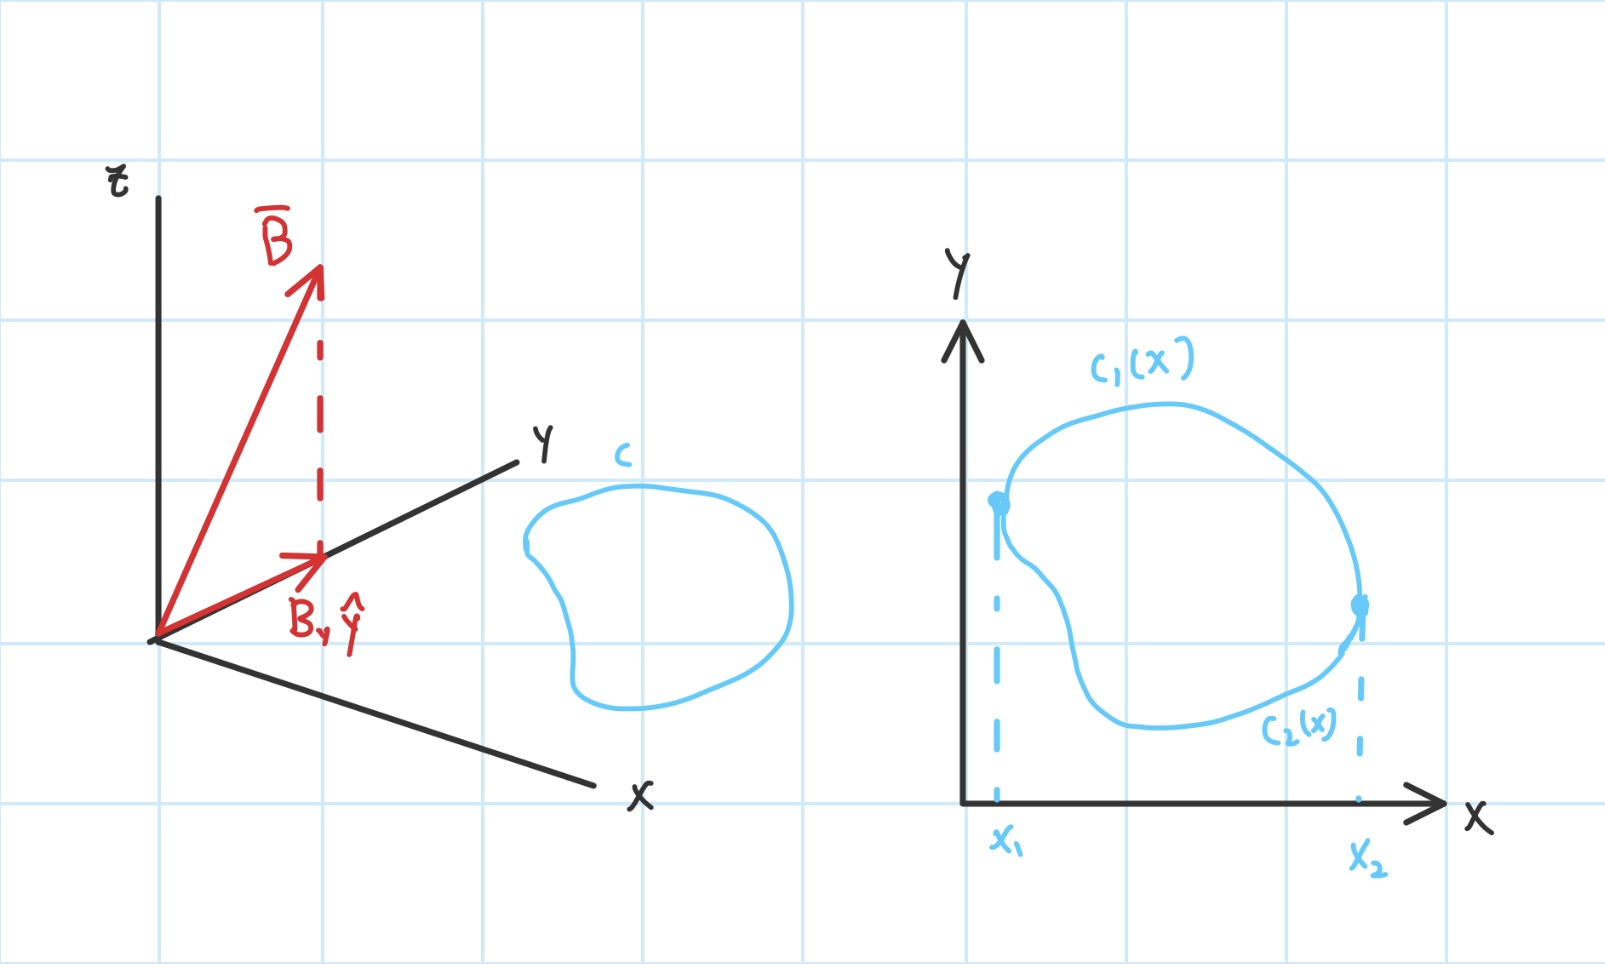
\includegraphics[width=80mm]{IMG_0189.jpg}
        \caption{Illustration of Setup}
    \end{center}
\end{figure}

Given uniform magnetic field $\bar{B}$ that is orthogonal to $\hat{x}$ (assume only the y-component $B_y\hat{y}$ is affecting the loop), 
and suppose a simple loop $c:[0,1]\rightarrow \mathbb{R}^3$ lies on the xy plane. Which, on the xy plane,
the loop can be decompose into upper part $c_1(x)$ and lower part $c_2(x)$ two functions (where $x_1$ and $x_2$ are the min and max value of the x-coordinate of $c(t)$).

Suppose the loop has a current $I$ going counterclockwise (if it's going in clockwise direction, take negative current $-I$ instead).

\hfill

Which, $c_1$ has current going to the left, for any small change in x-value $dx$, the change in space is given by
$d\bar{r_1} = (dx, c_1'(x)dx,0)$, which the current is given by $-Id\bar{r_1} = (-Idx, -Ic_1'(x)dx,0)$.

Then, for each position $x\in [x_1,x_2]$, the force on the currenct component of $c_1$ is given as $-Id\bar{r}\times B_y\hat{y}$,
so the torque is given by $d\bar{N}_1=c_1(x)\hat{y}\times (-Id\bar{r_1}\times B_y\hat{y})$. (Note: $c_1(x)\hat{y}$ is the displacement of the point away from x-axis, the rotation axis).
It can be simplified further as:
$$d\bar{N}_1=-IB_yc_1(x)(\hat{y}\times (d\bar{r_1}\times \hat{y}) = -IB_yc_1(x)((\hat{y}\cdot\hat{y})d\bar{r_1}-(\hat{y}\cdot d\bar{r_1})\hat{y})$$
$$ = -IB_yc_1(x)((dx,c_1'(x)dx,0)-c_1'(x)dx\hat{y})$$
$$ = -IB_yc_1(x)(dx,0,0)$$

\hfill

On the other hand, $c_2$ has curent going to the right, for any small change in x-value $dx$, the change in space is given by 
$d\bar{r_2}=(dx,c_2'(x)dx,0)$, so the current is given by $Id\bar{r_2} = (Idx,Ic_2'(x)dx,0)$.

Then, for each position $x\in[x_1,x_2]$, the force on the current component of $c_2$ is given as $Id\bar{r_2}\times B_y\hat{y}$,
so the torque is given by $d\bar{N}_2 = c_2(x)\hat{y}\times (Id\bar{r_2}\times B_y\hat{y})$. Which can be simplified as:
$$d\bar{N}_2 = IB_yc_2(x)(\hat{y}\times(d\bar{r_2}\times \hat{y})) = IB_yc_2(x)((\hat{y}\cdot\hat{y})d\bar{r_2}-(\hat{y}\cdot d\bar{r_2})\hat{y})$$
$$=IB_yc_2(x)((dx,c_2'(x)dx,0)-(c_2'(x)dx)\hat{y})$$
$$=IB_yc_2(x)(dx,0,0)$$

\hfill

Combining both torques, for the current elements on $x\in[x_1,x_2]$, the torque is given by:
$$d\bar{N}=d\bar{N}_1+d\bar{N}_2 = IB_y(c_2(x)-c_1(x))(dx,0,0) = (-IB_y(c_1(x)-c_2(x))dx,0,0)$$
Thus, the total torque is given by:
$$\bar{N}=\int_{x_1}^{x_2}d\bar{N} = \left(\int_{x_1}^{x_2}-IB_y(c_1(x)-c_2(x))dx,0,0\right)$$
Which, $a=\int_{x_1}^{x_2}(c_1(x)-c_2(x))dx$ is the enclosed area of the planar loop, which the torque is given as:
$$\bar{N}=(-IB_ya,0,0)$$

\hfill

\textbf{Torque and Magnetic Moment:}

From the above assumption, the current is going counterclockwise, so the normal vector of the enclosed area is going upward based on right-hand rule.
Thus, the magnetic moment is given by $\bar{m}=Ia\hat{z}$, where $I$ is the current and $a$ is the enclosed area.

Now, since the magnetic field $\bar{B}=B_y\hat{y}+B_z\hat{z}$ (since it is orthogonal to the x-axis, which is solely in yz plane). Then:
$$\bar{m}\times \bar{B}=(Ia\hat{z})\times(B_y\hat{y}+B_z\hat{z}) = IaB_y(\hat{z}\times \hat{y}) = -IaB_y\hat{x}=\bar{N}$$
(Note: since $\hat{z}\times\hat{z}=\bar{0}$, and $\hat{z}\times\hat{y}=-\hat{y}\times\hat{z}=-\hat{x}$, the above equation is true).
Thus, we can conclude that $\bar{m}\times\bar{B}=\bar{N}$, under the given condition.

\hfill

\textbf{Total Force:}

Recall from the first part, the force on the current component of $c_1$ is given as: 
$$d\bar{F}_1=-Id\bar{r_1}\times B_y\hat{y} = -IB_y(dx,c_1'(x)dx,0)\times\hat{y} = -IB_ydx\hat{x}\times \hat{y} = -IB_ydx\hat{z}$$
Also, the force on the current component of $c_2$ is given as:
$$d\bar{F}_2 = Id\bar{r_2}\times B_y\hat{y}=IB_y(dx,c2'(x)dx,0)\times \hat{y}=IB_ydx\hat{x}\times\hat{y}=IB_ydx\hat{z}$$
Which, the force on the components with x-coordinate $x\in[x_1,x_2]$ is given by $d\bar{F} = d\bar{F_1}+d\bar{F_2}$, 
so the force on the whole loop is given as follow:
$$\bar{F} = \int_{x_1}^{x_2}d\bar{F}=\int_{x_1}^{x_2}(-IB_ydx\hat{z}+IB_ydx\hat{z}) = \hat{z}\int_{x_1}^{x_2}0dx = \bar{0}$$
Thus, the total force on the loop is $\bar{0}$, no force is exerted.

\break

\section*{4}
\begin{myBox}[]{}
    \begin{question}
        A current carrying, plane loop of conductor generates a magnetic induction $\hat{B}(\hat{r})$. A current-
        element at some point P on the conductor interacts with the ~B-field which is created by other
        current-elements. Calculate the total force which the conductor loop exerts on itself. Consider
        the conductor as a ’thread of current’.
    \end{question}
\end{myBox}

\textbf{Pf:}

Suppose the plane loop of conductor is in circular shape, and for arbitrary point $P$, set the angle to be at $\theta=0$.
\begin{figure}[h!]
    \begin{center}
        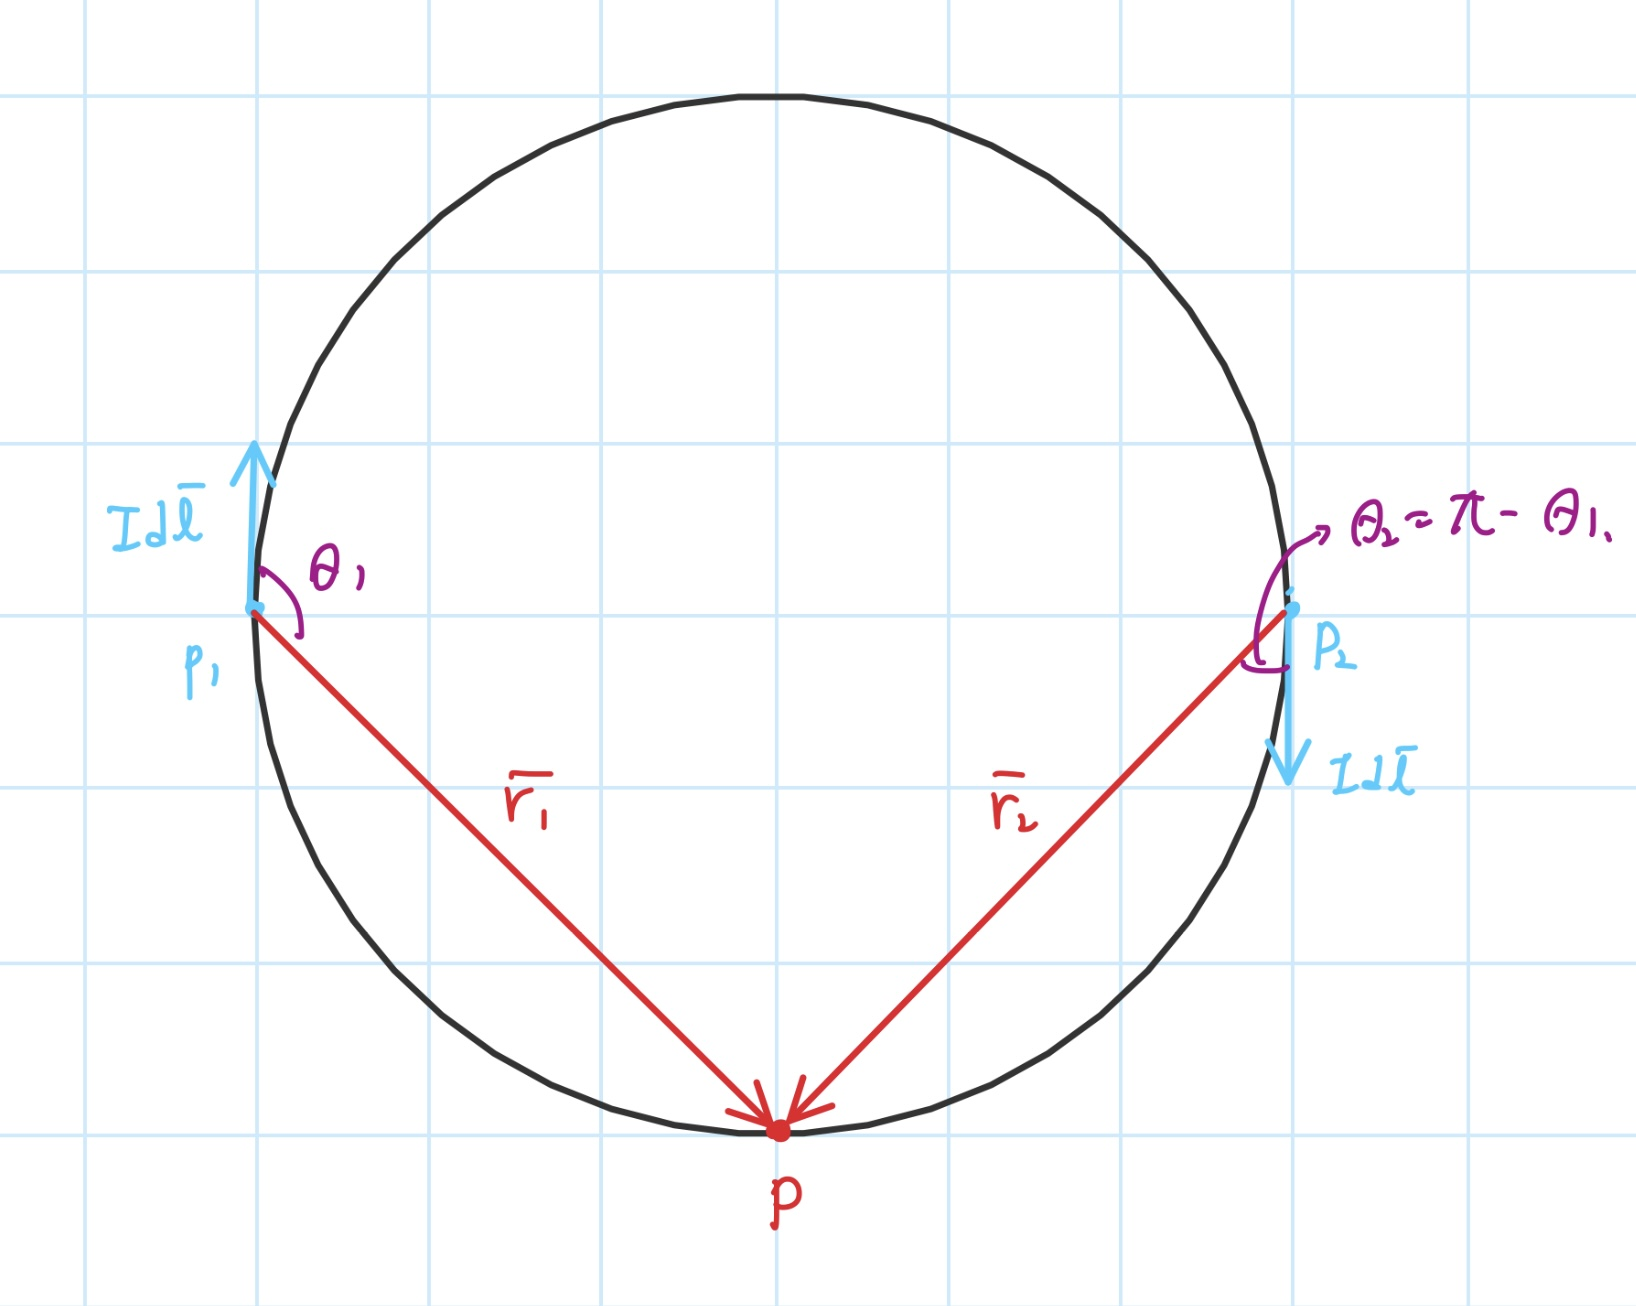
\includegraphics[width=60mm]{IMG_0190.jpg}
        \caption{Illustration of Setup}
    \end{center}
\end{figure}
Then, for the point $P_1$ (on angle $-\theta$) and the point $P_2$ (on angle $\theta$), they're the points that're symmetric along the vertical axis at the center,
so they have the same distance away from point $P$ (or, $r_1=r_2$).
Which, based on the illustration, one can observe that given steady current $I$ and same amount of spacial change $dl$, the magnetic field strength on $P$ generated by $P_1$ and $P_2$,
are given as:
$$B_{P_1}(P) = |d\bar{l}|\cdot|\bar{r_1}|\cdot\sin(\theta_1) = dl\cdot r_1\sin(\theta_1)$$
$$B_{P_2}(P)=|d\bar{l}|\cdot|\bar{r_2}|\cdot\sin(\theta_2)=dl\cdot r_2\sin(\pi-\theta_1)=dl\cdot r_2\sin(\theta_1)$$
So, the two current components $P_1,P_2$ generate the same magnetic field strength.

However, based on Right Hand Rule, the field induced by $P_1$ is pointing into the page, while the field induced by $P_2$ is pointing out of the page.
So, $\bar{B_{P_1}}(P)$ and $\bar{B_{P_2}}(P)$ are two fields at point $P$, with the same magnitude but opposite direction, which the combined field on $P$ is $\bar{0}$.

\hfill

Now, since the circular loop is symmetric, then for all pairs of $P_1$ and $P_2$, the field induced on $P$ is always $\bar{0}$, then the total magnetic field at $P$
generated by other current components is in fact $\bar{0}$, implying the force on $P$ is $\bar{0}$.

\hfill

Finally, since the point $P$ is arbitary, then we can say the force component on each point $P$ is $\bar{0}$, which the net force is $\bar{0}$.

\end{document}